% Options for packages loaded elsewhere
\PassOptionsToPackage{unicode}{hyperref}
\PassOptionsToPackage{hyphens}{url}
%
\documentclass[
]{article}
\usepackage{amsmath,amssymb}
\usepackage{lmodern}
\usepackage{iftex}
\ifPDFTeX
  \usepackage[T1]{fontenc}
  \usepackage[utf8]{inputenc}
  \usepackage{textcomp} % provide euro and other symbols
\else % if luatex or xetex
  \usepackage{unicode-math}
  \defaultfontfeatures{Scale=MatchLowercase}
  \defaultfontfeatures[\rmfamily]{Ligatures=TeX,Scale=1}
\fi
% Use upquote if available, for straight quotes in verbatim environments
\IfFileExists{upquote.sty}{\usepackage{upquote}}{}
\IfFileExists{microtype.sty}{% use microtype if available
  \usepackage[]{microtype}
  \UseMicrotypeSet[protrusion]{basicmath} % disable protrusion for tt fonts
}{}
\makeatletter
\@ifundefined{KOMAClassName}{% if non-KOMA class
  \IfFileExists{parskip.sty}{%
    \usepackage{parskip}
  }{% else
    \setlength{\parindent}{0pt}
    \setlength{\parskip}{6pt plus 2pt minus 1pt}}
}{% if KOMA class
  \KOMAoptions{parskip=half}}
\makeatother
\usepackage{xcolor}
\usepackage[margin=1in]{geometry}
\usepackage{color}
\usepackage{fancyvrb}
\newcommand{\VerbBar}{|}
\newcommand{\VERB}{\Verb[commandchars=\\\{\}]}
\DefineVerbatimEnvironment{Highlighting}{Verbatim}{commandchars=\\\{\}}
% Add ',fontsize=\small' for more characters per line
\usepackage{framed}
\definecolor{shadecolor}{RGB}{248,248,248}
\newenvironment{Shaded}{\begin{snugshade}}{\end{snugshade}}
\newcommand{\AlertTok}[1]{\textcolor[rgb]{0.94,0.16,0.16}{#1}}
\newcommand{\AnnotationTok}[1]{\textcolor[rgb]{0.56,0.35,0.01}{\textbf{\textit{#1}}}}
\newcommand{\AttributeTok}[1]{\textcolor[rgb]{0.77,0.63,0.00}{#1}}
\newcommand{\BaseNTok}[1]{\textcolor[rgb]{0.00,0.00,0.81}{#1}}
\newcommand{\BuiltInTok}[1]{#1}
\newcommand{\CharTok}[1]{\textcolor[rgb]{0.31,0.60,0.02}{#1}}
\newcommand{\CommentTok}[1]{\textcolor[rgb]{0.56,0.35,0.01}{\textit{#1}}}
\newcommand{\CommentVarTok}[1]{\textcolor[rgb]{0.56,0.35,0.01}{\textbf{\textit{#1}}}}
\newcommand{\ConstantTok}[1]{\textcolor[rgb]{0.00,0.00,0.00}{#1}}
\newcommand{\ControlFlowTok}[1]{\textcolor[rgb]{0.13,0.29,0.53}{\textbf{#1}}}
\newcommand{\DataTypeTok}[1]{\textcolor[rgb]{0.13,0.29,0.53}{#1}}
\newcommand{\DecValTok}[1]{\textcolor[rgb]{0.00,0.00,0.81}{#1}}
\newcommand{\DocumentationTok}[1]{\textcolor[rgb]{0.56,0.35,0.01}{\textbf{\textit{#1}}}}
\newcommand{\ErrorTok}[1]{\textcolor[rgb]{0.64,0.00,0.00}{\textbf{#1}}}
\newcommand{\ExtensionTok}[1]{#1}
\newcommand{\FloatTok}[1]{\textcolor[rgb]{0.00,0.00,0.81}{#1}}
\newcommand{\FunctionTok}[1]{\textcolor[rgb]{0.00,0.00,0.00}{#1}}
\newcommand{\ImportTok}[1]{#1}
\newcommand{\InformationTok}[1]{\textcolor[rgb]{0.56,0.35,0.01}{\textbf{\textit{#1}}}}
\newcommand{\KeywordTok}[1]{\textcolor[rgb]{0.13,0.29,0.53}{\textbf{#1}}}
\newcommand{\NormalTok}[1]{#1}
\newcommand{\OperatorTok}[1]{\textcolor[rgb]{0.81,0.36,0.00}{\textbf{#1}}}
\newcommand{\OtherTok}[1]{\textcolor[rgb]{0.56,0.35,0.01}{#1}}
\newcommand{\PreprocessorTok}[1]{\textcolor[rgb]{0.56,0.35,0.01}{\textit{#1}}}
\newcommand{\RegionMarkerTok}[1]{#1}
\newcommand{\SpecialCharTok}[1]{\textcolor[rgb]{0.00,0.00,0.00}{#1}}
\newcommand{\SpecialStringTok}[1]{\textcolor[rgb]{0.31,0.60,0.02}{#1}}
\newcommand{\StringTok}[1]{\textcolor[rgb]{0.31,0.60,0.02}{#1}}
\newcommand{\VariableTok}[1]{\textcolor[rgb]{0.00,0.00,0.00}{#1}}
\newcommand{\VerbatimStringTok}[1]{\textcolor[rgb]{0.31,0.60,0.02}{#1}}
\newcommand{\WarningTok}[1]{\textcolor[rgb]{0.56,0.35,0.01}{\textbf{\textit{#1}}}}
\usepackage{graphicx}
\makeatletter
\def\maxwidth{\ifdim\Gin@nat@width>\linewidth\linewidth\else\Gin@nat@width\fi}
\def\maxheight{\ifdim\Gin@nat@height>\textheight\textheight\else\Gin@nat@height\fi}
\makeatother
% Scale images if necessary, so that they will not overflow the page
% margins by default, and it is still possible to overwrite the defaults
% using explicit options in \includegraphics[width, height, ...]{}
\setkeys{Gin}{width=\maxwidth,height=\maxheight,keepaspectratio}
% Set default figure placement to htbp
\makeatletter
\def\fps@figure{htbp}
\makeatother
\setlength{\emergencystretch}{3em} % prevent overfull lines
\providecommand{\tightlist}{%
  \setlength{\itemsep}{0pt}\setlength{\parskip}{0pt}}
\setcounter{secnumdepth}{-\maxdimen} % remove section numbering
\ifLuaTeX
  \usepackage{selnolig}  % disable illegal ligatures
\fi
\IfFileExists{bookmark.sty}{\usepackage{bookmark}}{\usepackage{hyperref}}
\IfFileExists{xurl.sty}{\usepackage{xurl}}{} % add URL line breaks if available
\urlstyle{same} % disable monospaced font for URLs
\hypersetup{
  pdftitle={drugs},
  pdfauthor={Nicole Ayala},
  hidelinks,
  pdfcreator={LaTeX via pandoc}}

\title{drugs}
\author{Nicole Ayala}
\date{2023-03-19}

\begin{document}
\maketitle

\#\#In this Tidy Tuesday, I will be using a series of packages to create
individual linear plots for 4 different types of diseases and see their
correlation in how many medications have been authorised for it in the
past 20 years.

\#\#\#Loading the Libraries

\begin{Shaded}
\begin{Highlighting}[]
\DocumentationTok{\#\#\# Load Libraries }\AlertTok{\#\#\#}
\FunctionTok{library}\NormalTok{(tidyverse)}
\FunctionTok{library}\NormalTok{(here)}
\FunctionTok{library}\NormalTok{(tidytuesdayR)}
\FunctionTok{library}\NormalTok{(svglite)}
\FunctionTok{library}\NormalTok{(colorspace)}
\FunctionTok{library}\NormalTok{(tidyr)}
\FunctionTok{library}\NormalTok{(dplyr)}
\FunctionTok{library}\NormalTok{(beyonce)}
\FunctionTok{library}\NormalTok{(ggplot2)}
\end{Highlighting}
\end{Shaded}

\hypertarget{loading-the-data}{%
\subsubsection{Loading the Data}\label{loading-the-data}}

\begin{Shaded}
\begin{Highlighting}[]
\DocumentationTok{\#\#\# Load the Data }\AlertTok{\#\#\#}
\NormalTok{drugs }\OtherTok{\textless{}{-}}\NormalTok{ readr}\SpecialCharTok{::}\FunctionTok{read\_csv}\NormalTok{(}\StringTok{\textquotesingle{}https://raw.githubusercontent.com/rfordatascience/tidytuesday/master/data/2023/2023{-}03{-}14/drugs.csv\textquotesingle{}}\NormalTok{)}
\FunctionTok{glimpse}\NormalTok{(drugs) }\CommentTok{\# viewing data}
\end{Highlighting}
\end{Shaded}

\begin{verbatim}
## Rows: 1,988
## Columns: 28
## $ category                                    <chr> "human", "human", "human",~
## $ medicine_name                               <chr> "Adcetris", "Nityr", "Ebva~
## $ therapeutic_area                            <chr> "Lymphoma, Non-Hodgkin;  H~
## $ common_name                                 <chr> "brentuximab vedotin", "ni~
## $ active_substance                            <chr> "brentuximab vedotin", "ni~
## $ product_number                              <chr> "002455", "004582", "00457~
## $ patient_safety                              <lgl> FALSE, FALSE, FALSE, FALSE~
## $ authorisation_status                        <chr> "authorised", "authorised"~
## $ atc_code                                    <chr> "L01XC12", "A16AX04", NA, ~
## $ additional_monitoring                       <lgl> FALSE, FALSE, TRUE, TRUE, ~
## $ generic                                     <lgl> FALSE, TRUE, FALSE, FALSE,~
## $ biosimilar                                  <lgl> FALSE, FALSE, FALSE, FALSE~
## $ conditional_approval                        <lgl> FALSE, FALSE, FALSE, FALSE~
## $ exceptional_circumstances                   <lgl> FALSE, FALSE, TRUE, FALSE,~
## $ accelerated_assessment                      <lgl> FALSE, FALSE, FALSE, FALSE~
## $ orphan_medicine                             <lgl> TRUE, FALSE, TRUE, FALSE, ~
## $ marketing_authorisation_date                <date> 2012-10-25, 2018-07-26, 2~
## $ date_of_refusal_of_marketing_authorisation  <date> NA, NA, NA, NA, NA, NA, N~
## $ marketing_authorisation_holder_company_name <chr> "Takeda Pharma A/S", "Cycl~
## $ pharmacotherapeutic_group                   <chr> "Antineoplastic agents", "~
## $ date_of_opinion                             <date> 2012-07-19, 2018-05-31, 2~
## $ decision_date                               <date> 2022-11-17, 2023-03-10, 2~
## $ revision_number                             <dbl> 34, 4, 2, 3, 30, 24, 4, 18~
## $ condition_indication                        <chr> "Hodgkin lymphomaAdcetris ~
## $ species                                     <chr> NA, NA, NA, NA, NA, NA, NA~
## $ first_published                             <dttm> 2018-07-25 13:58:00, 2018~
## $ revision_date                               <dttm> 2023-03-13 11:52:00, 2023~
## $ url                                         <chr> "https://www.ema.europa.eu~
\end{verbatim}

\begin{Shaded}
\begin{Highlighting}[]
\NormalTok{q11 }\OtherTok{\textless{}{-}} \FunctionTok{qualitative\_hcl}\NormalTok{(}\DecValTok{11}\NormalTok{, }\StringTok{"Dark2"}\NormalTok{) }\CommentTok{\# changing the color name}

\DocumentationTok{\#\#\# cleaning therapeutic areas {-} selecting only one}
\NormalTok{ parkinson }\OtherTok{\textless{}{-}}\NormalTok{ drugs }\SpecialCharTok{\%\textgreater{}\%} \CommentTok{\# looking at cleaning this data}
 \FunctionTok{filter}\NormalTok{(}\SpecialCharTok{!}\FunctionTok{is.na}\NormalTok{(therapeutic\_area)) }\SpecialCharTok{\%\textgreater{}\%}
  \FunctionTok{count}\NormalTok{(therapeutic\_area, category) }\SpecialCharTok{\%\textgreater{}\%} \CommentTok{\# only counting category and therap{-}areas }
  \FunctionTok{arrange}\NormalTok{() }\SpecialCharTok{\%\textgreater{}\%} \CommentTok{\# arranges in ascending order}
  \FunctionTok{filter}\NormalTok{(}\FunctionTok{str\_detect}\NormalTok{(therapeutic\_area, }\StringTok{"Parkinson Disease"}\NormalTok{)) }\CommentTok{\#  detecting only parkinsons}
 
\NormalTok{ medname }\OtherTok{\textless{}{-}}\NormalTok{ drugs }\SpecialCharTok{\%\textgreater{}\%}  \CommentTok{\# looking at names}
  \FunctionTok{count}\NormalTok{(medicine\_name) }\CommentTok{\# count fo each medicine name}
   
\NormalTok{ activesubst }\OtherTok{\textless{}{-}}\NormalTok{ drugs }\SpecialCharTok{\%\textgreater{}\%} \CommentTok{\# looking at substances}
  \FunctionTok{count}\NormalTok{(active\_substance) }\CommentTok{\# count of each active substance}
 
\NormalTok{parkinson\_df}\OtherTok{\textless{}{-}}\NormalTok{drugs }\SpecialCharTok{\%\textgreater{}\%} 
  \FunctionTok{select}\NormalTok{(therapeutic\_area, active\_substance) }\SpecialCharTok{\%\textgreater{}\%} \CommentTok{\# selecting two factors:active substance and therapeutic data}
  \FunctionTok{mutate}\NormalTok{(}\AttributeTok{active\_substance =} \FunctionTok{str\_to\_sentence}\NormalTok{(active\_substance)) }\CommentTok{\# convert to sentence case}

\NormalTok{parkinson\_df}\OtherTok{\textless{}{-}}\NormalTok{parkinson\_df }\SpecialCharTok{\%\textgreater{}\%}  \CommentTok{\# piping to itself makes it stronger to break}
  \FunctionTok{group\_by}\NormalTok{(therapeutic\_area, active\_substance) }\SpecialCharTok{\%\textgreater{}\%} \CommentTok{\# grouping therapeutic area and active substance together}
  \FunctionTok{mutate}\NormalTok{(}\AttributeTok{drug\_number =} \FunctionTok{row\_number}\NormalTok{()) }\SpecialCharTok{\%\textgreater{}\%} \CommentTok{\# amount of drugs is correlated to rows}
  \FunctionTok{ungroup}\NormalTok{() }
 
\NormalTok{semijoindrug}\OtherTok{\textless{}{-}}\NormalTok{ drugs }\SpecialCharTok{\%\textgreater{}\%} 
  \FunctionTok{semi\_join}\NormalTok{(activesubst, }\AttributeTok{by =} \StringTok{"active\_substance"}\NormalTok{) }\SpecialCharTok{\%\textgreater{}\%}  \CommentTok{\# active substances specific to parkinson within the entire dataset including active susbstances}
  \FunctionTok{semi\_join}\NormalTok{(parkinson, }\AttributeTok{by =} \StringTok{"therapeutic\_area"}\NormalTok{) }\SpecialCharTok{\%\textgreater{}\%} \CommentTok{\# tried out the semi joining of the therapeutic area and being filtered out to parkinson only}
  \FunctionTok{count}\NormalTok{(active\_substance, therapeutic\_area) }\SpecialCharTok{\%\textgreater{}\%} \CommentTok{\# wanna see the active substance given per therapeutic area/ disease}
  \FunctionTok{filter}\NormalTok{(therapeutic\_area }\SpecialCharTok{==} \StringTok{"Parkinson Disease"}\NormalTok{) }\CommentTok{\# already filtered out but to be structured I stayed consistent}
\end{Highlighting}
\end{Shaded}

\begin{Shaded}
\begin{Highlighting}[]
\DocumentationTok{\#\#\# Plotting Time}
  \FunctionTok{ggplot}\NormalTok{(}\AttributeTok{data=}\NormalTok{semijoindrug,}
    \FunctionTok{aes}\NormalTok{(}\AttributeTok{x =}\NormalTok{ active\_substance,     }\CommentTok{\# x axis is the active substance}
        \AttributeTok{y=}\NormalTok{n,  }\CommentTok{\# number of active sub/drugs}
        \AttributeTok{fill =}\NormalTok{active\_substance)) }\SpecialCharTok{+}  \CommentTok{\#y axis is number of drugs, fill is active substance}
  \FunctionTok{geom\_col}\NormalTok{() }\SpecialCharTok{+}  \CommentTok{\# bar plot}
  \FunctionTok{labs}\NormalTok{(}
    \AttributeTok{title =} \FunctionTok{str\_wrap}\NormalTok{(}\StringTok{"Analysis of the Various Medications Used in Both Humanitarian and Veterinary Agencies for Parkinson Disease Within Europe"}\NormalTok{,}\DecValTok{2500}\NormalTok{),}\CommentTok{\# just the title}
    \AttributeTok{subtitle =} \FunctionTok{str\_wrap}\NormalTok{ (}\StringTok{"Demonstrates Various Active Substances for Parkinsons"}\NormalTok{,}\DecValTok{150}\NormalTok{),   }\CommentTok{\# subtitle}
    \AttributeTok{caption =} \StringTok{" NAA | Data: European Drug Development"}\NormalTok{, }\CommentTok{\# caption}
    \AttributeTok{x =} \StringTok{" Active Substances "}\NormalTok{, }\CommentTok{\# x axis}
    \AttributeTok{y =}\StringTok{"Recurrence of Active Substances"}\NormalTok{, }\CommentTok{\# y axis}
    \AttributeTok{fill =}\StringTok{"active substances"}\NormalTok{) }\SpecialCharTok{+} \CommentTok{\# fill active substances}
  \FunctionTok{scale\_fill\_brewer}\NormalTok{(}\AttributeTok{palette =} \StringTok{"Spectral"}\NormalTok{) }\SpecialCharTok{+}   \CommentTok{\# Color scheme for the categories}
  \FunctionTok{coord\_flip}\NormalTok{() }\SpecialCharTok{+} \CommentTok{\# invert the x axis and y axis to read the substances}
  \FunctionTok{scale\_size}\NormalTok{(}\AttributeTok{range =} \FunctionTok{c}\NormalTok{(.}\DecValTok{1}\NormalTok{, .}\DecValTok{2}\NormalTok{)) }\SpecialCharTok{+} \CommentTok{\# small scale}
  \FunctionTok{theme\_light}\NormalTok{() }\SpecialCharTok{+} \CommentTok{\# very light white theme}
  \FunctionTok{theme}\NormalTok{(}\AttributeTok{plot.title =} \FunctionTok{element\_text}\NormalTok{(}\AttributeTok{hjust =}\NormalTok{ .}\DecValTok{2}\NormalTok{,}\AttributeTok{vjust =} \SpecialCharTok{{-}}\FloatTok{1.20}\NormalTok{, }\AttributeTok{size =} \DecValTok{15}\NormalTok{, }\AttributeTok{color =} \StringTok{"seagreen4"}\NormalTok{), }\CommentTok{\# changes the color and size of the title}
        \AttributeTok{plot.subtitle =} \FunctionTok{element\_text}\NormalTok{(}\AttributeTok{hjust =}\NormalTok{ .}\DecValTok{2}\NormalTok{,}\AttributeTok{vjust =} \SpecialCharTok{{-}}\FloatTok{1.20}\NormalTok{, }\AttributeTok{size =} \DecValTok{10}\NormalTok{, }\AttributeTok{color =} \StringTok{"paleturquoise3"}\NormalTok{), }\CommentTok{\# changes the color and size of the subtitle}
        \AttributeTok{plot.background =} \FunctionTok{element\_rect}\NormalTok{(}\AttributeTok{fill =} \StringTok{\textquotesingle{}white\textquotesingle{}}\NormalTok{, }\AttributeTok{color =} \StringTok{\textquotesingle{}white\textquotesingle{}}\NormalTok{)) }\CommentTok{\# just to fill in the background, behind the gridlines}
\end{Highlighting}
\end{Shaded}

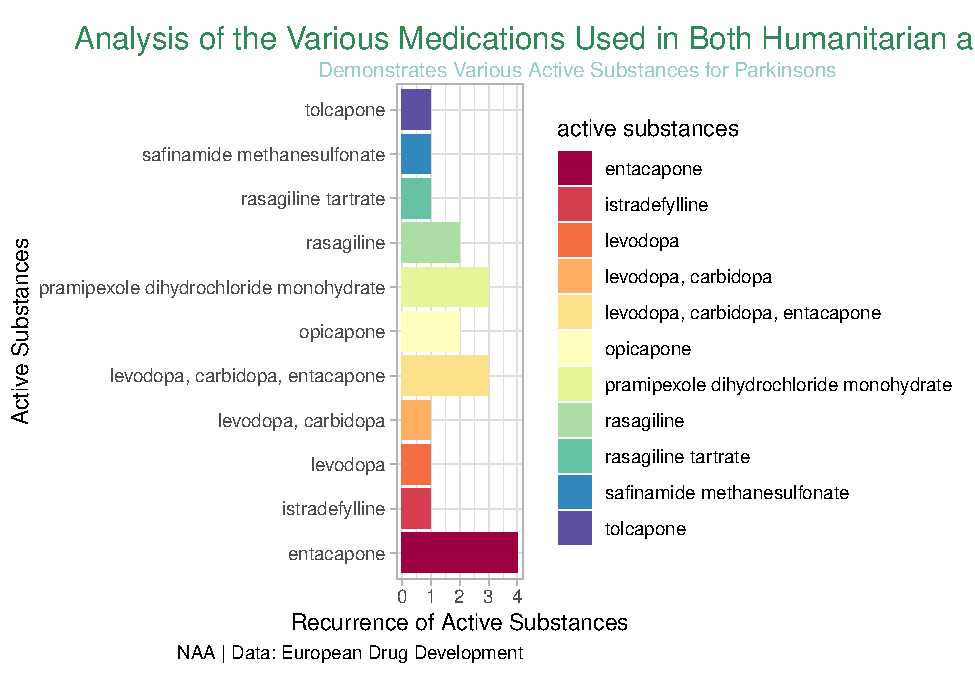
\includegraphics{../Output/unnamed-chunk-3-1.pdf}

\begin{Shaded}
\begin{Highlighting}[]
\FunctionTok{ggsave}\NormalTok{(}\FunctionTok{here}\NormalTok{(}\StringTok{"Fifth Tidy Tuesday"}\NormalTok{,}\StringTok{"Output"}\NormalTok{,}\StringTok{"5thTidyTuesdayDrugsPlot.png"}\NormalTok{),}\CommentTok{\# names and saves ggplot}
       \AttributeTok{width =} \DecValTok{15}\NormalTok{, }\AttributeTok{height =} \DecValTok{10}\NormalTok{)}\CommentTok{\# adjust size of graph in inches}
\end{Highlighting}
\end{Shaded}

```

\end{document}
